\chapter{Monitoring}
We willen de verschillende applicaties die we ontwikkelen monitoren zodat we kunnen waarborgen dat de applicaties correct werken, en waar nodig snel inzichtelijk hebben waar we verbeteringen kunnen doorvoeren.

Het monitoren van de applicaties kunnen we op verschillende manieren doen. Dit begint al bij het bouwen van de applicatie naar de ontwikkel omgeving. Zoals eerder reeds aangegeven in dit document maken we gebruik van verschillende maven profielen om de applicatie te testen. Aan de hand van deze profielen kunnen we bijvoorbeeld automatisch unit tests en integratie tests uitvoeren. Dit is voor ons de eerste manier om achter eventuele fouten binnen de applicatie te komen.
Tevens gebruiken we Sentry om eventuele foutmeldingen op te kunnen sporen in de applciatie nadat deze gedeployed is.

\section{Performance van de applicaties}
Daarnaast willen we graag weten wat de perfomance is van onze applicaties. Hiermee doelen we bijvoorbeeld op de responsetijd om een verzoek te verwerken. Afhankelijk van de requirements, kan de responsetijd per onderdeel afwijken. Denk bijvoorbeeld aan de responsetijd voor het verzoek vanaf een website, of de responsetijd voor het verwerken van voertuiglocaties.
De performance van de applicaties kunnen we voor een deel tijdens het testen meten. Zo kunnen we bijvoorbeelde grote hoeveelheden verkeer naar de applicaties simuleren waardoor we een beter inzicht kunnen krijgen in de performance van de applicaties.
Daarnaast willen we periodiek performance testen uitvoeren op de productie omgeving.

\section{Performance van de hardware}
Onder de performance valt echter ook de hardware die gebruikt wordt. We willen namelijk weten hoeveel resources er gebruikt worden voor een applicatie zodat we, wanneer nodig, de beschikbare resources kunnen bij- of afschalen.
De verschillende applicaties worden beschikbaar gesteld in Infralab. Aangezien deze omgeving draait op VMWare vSphere, is er reeds een monitoring tool aanwezig om het CPU gebruik, Geheugen gebruikt en netwerk gebruikt te monitoren.
\newline
Sommige tooling (Sentry, Sonarqube, Artifactory) wordt niet gehost binnen Infralab, maar op een eigen server. Deze server maakt gebruik van Proxmox om verschillende machines te kunnen virtualiseren. Binnen Proxmox zijn tevens ook enkele monitorings gegevens zichtbaar zoals te zien is in figuur \ref{fig:proxmox}

\begin{figure}[H]
	\centering
	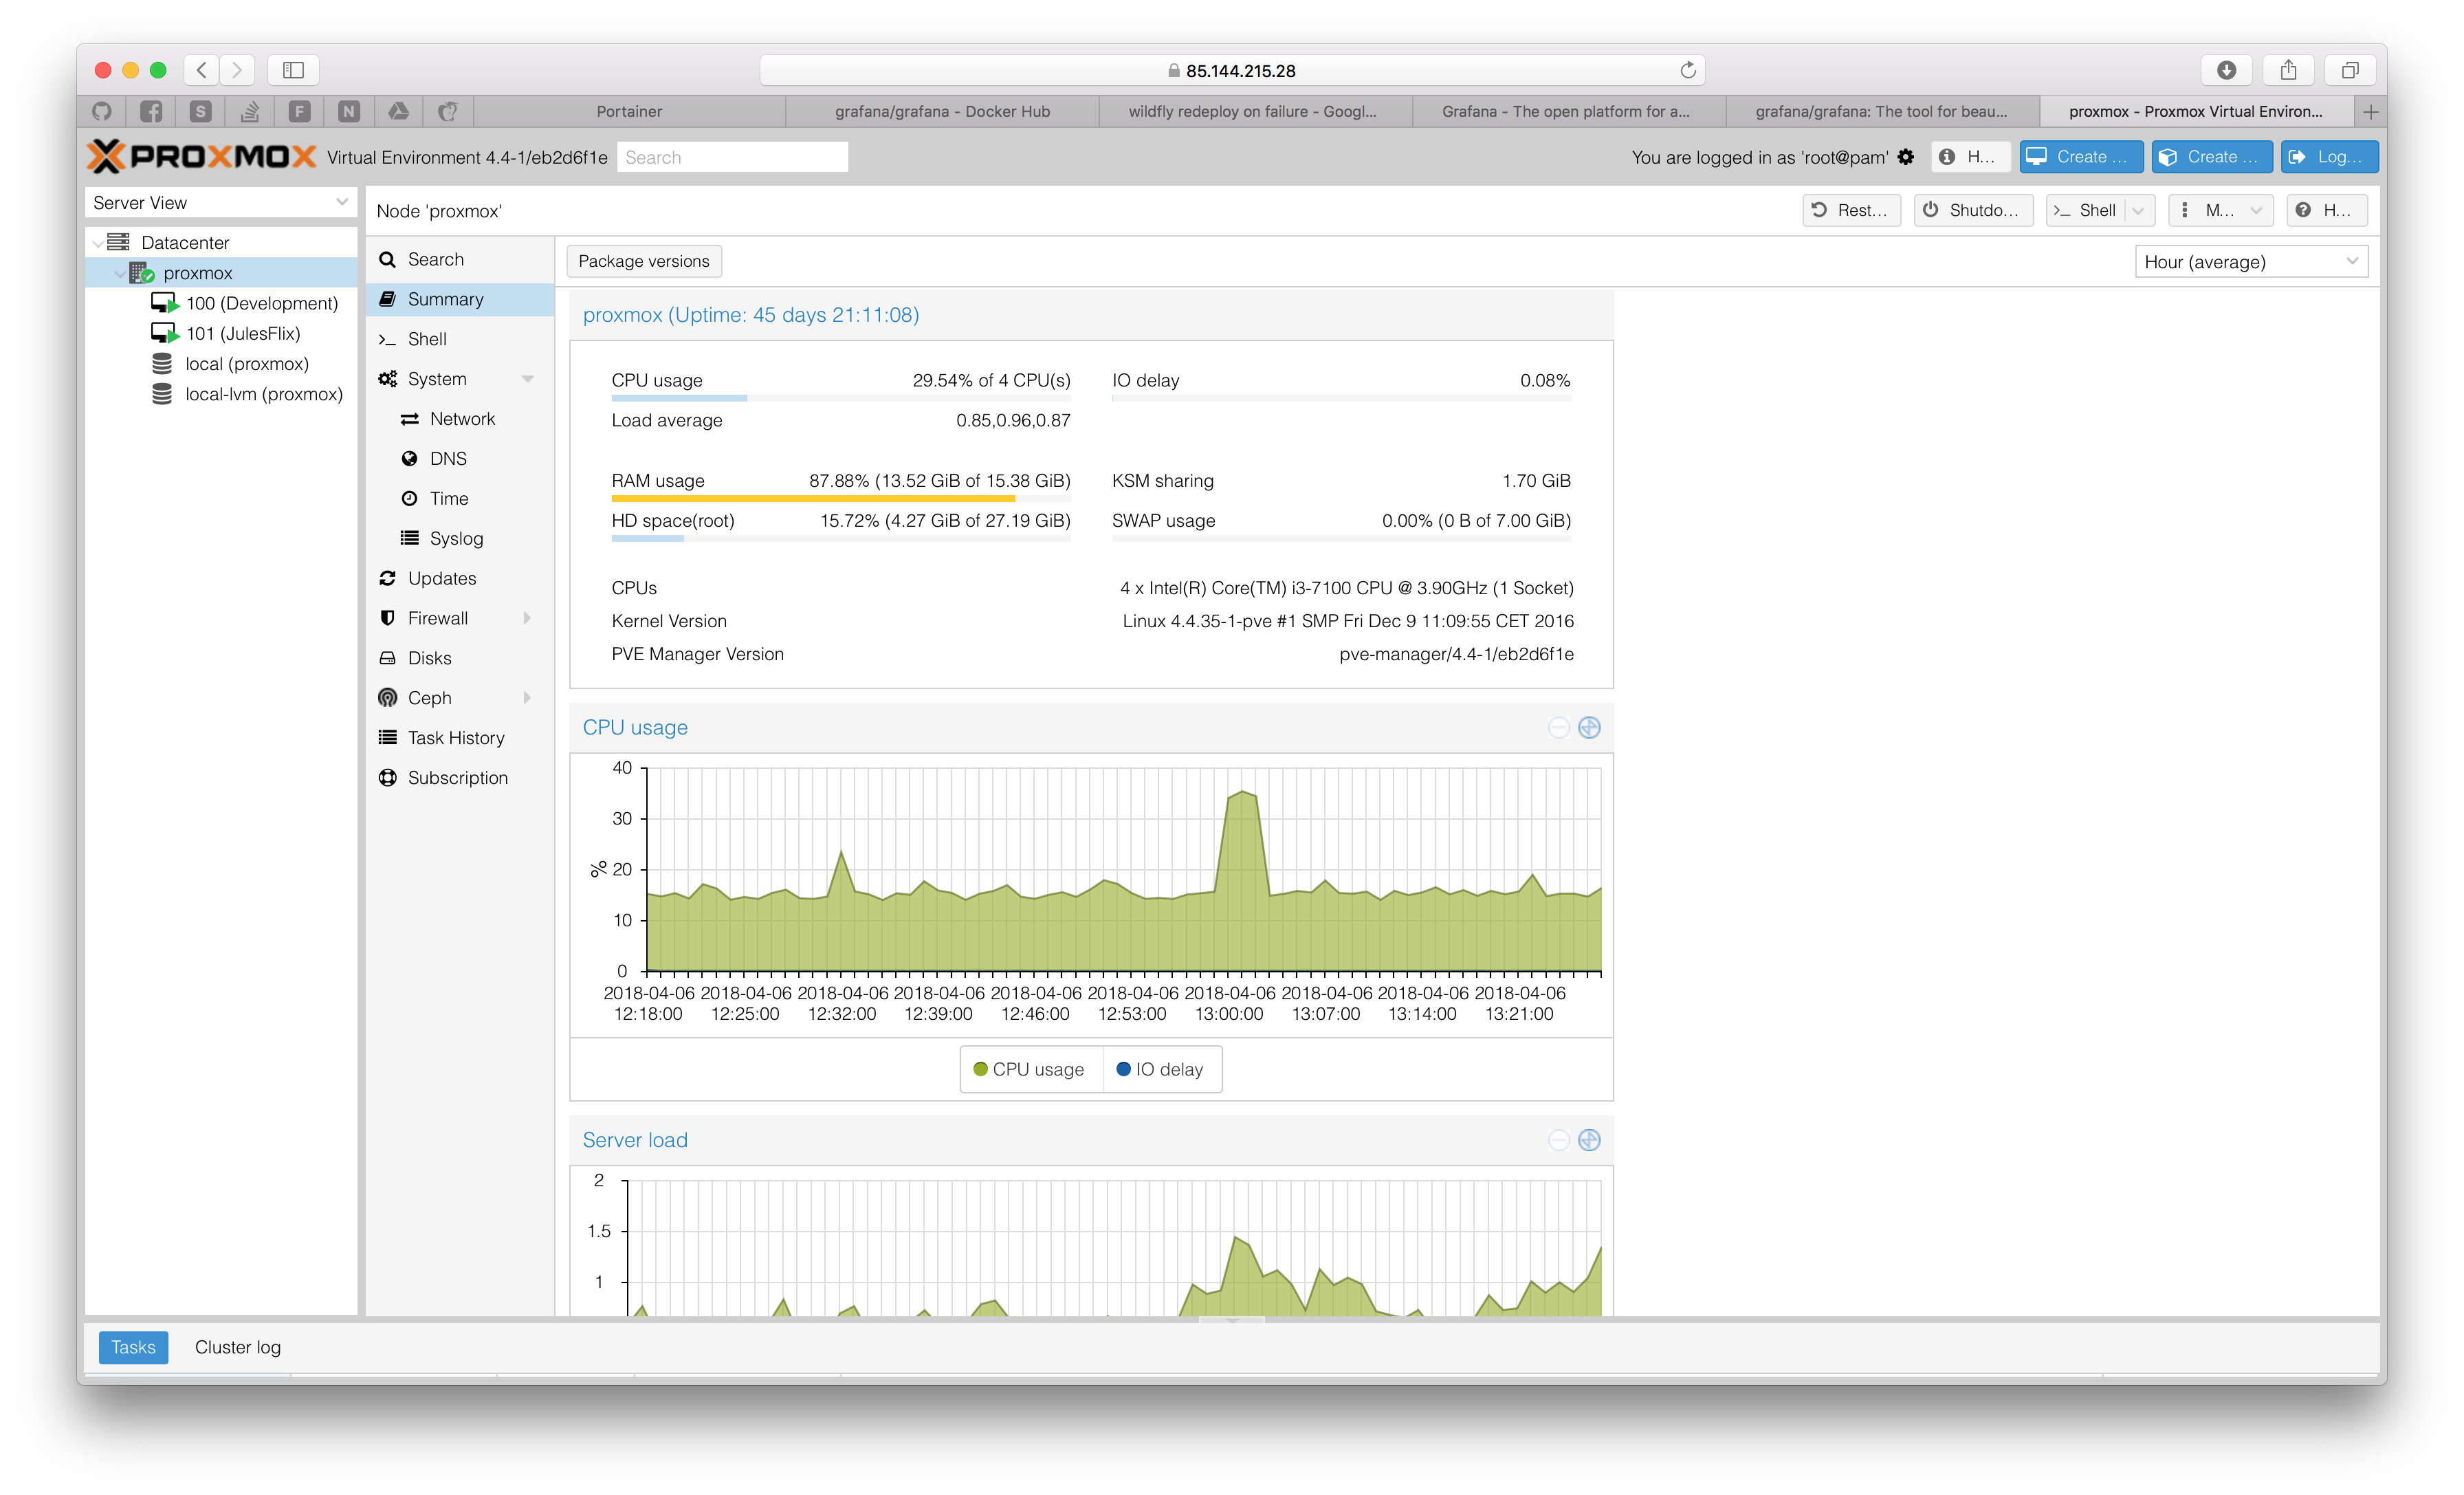
\includegraphics[width=0.95\textwidth]{img/proxmox.png}
	\caption{Proxmox statistieken voor alle beschikbare virtuele machines}
	\label{fig:proxmox}
\end{figure}

\section{Verwachtingen}
De verwachting is dat onze applicaties, en dan met name de registratie-verplaatsing, voornamelijk tijdens de spitsuren belast zullen worden. We willen dan ook monitoren wat de snelheid van de applicaties zijn tijdens de piekuren. Door performance metingen voor een bepaalde tijd uit te voeren, krijgen we meer inzicht op het gebruik van de applicaties waardoor we op een optimalere manier resources per applicatie kunnen toekennen. 

Momenteel zijn we bezig met een onderzoek naar welke tooling het beste ingezet kan worden om de verschillende applicaties te monitoren. Hierdoor is het op dit moment voor ons nog niet mogelijk om voorbeelden te laten zien en weten we nog niet of onze verwachtingen haalbaar zijn.
